Before actually starting to work on the dialogue itself, we decided on how a dialogue with the EllaVator should look like. \\

We came up with the following model: \\


\begin{figure} [ht]
\center{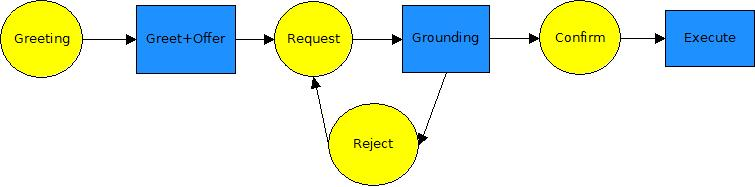
\includegraphics[scale=0.8, angle=0]{Dialogue_model.jpeg}}
\caption{A model for the Dialogue}
\label{fig: Dialogue flow}
\end{figure}

In the figure shown above commands from the user are marked in yellow, the answers from the EllaVator are marked in blue.
Here is a table giving example sentences for the states indicated by the figure above: \\


\begin{tabular}{|ll|}
\hline
Greeting & The user greets the Ellevator with a keyword \\
  & and thus activates the system.  \\
Greet + Offer & Hello, how can I help you? \\
Request & Take me to floor/room XY/ Name\_of\_a\_person \\
Grounding/Clarify & You'd like to be taken to ...?\\ 
 & I didn't get it, could you repeat that? \\
Confirm & Yes \\
Reject & No \\
Execute & Okay I shall now take you to ... \\ 
 & *here the elevator should also start the action of moving* \\
\hline 
\end{tabular}
\newline
Of course the actual system should be able to understand a variety of sentences and maybe alternate the answers but the dialogue itself can be kept as simple as it is shown in the graph.  \\

We thought about including some chatting with the user or small Easter eggs. 
We have therefore made measurements on how much time the average user spends in the elevator to determine how much time there is for the dialogue.
On average the elevator needed 40 seconds to go from the ground floor to the top and 21 seconds for going down. Opening the Doors takes 4 seconds, closing them 5.5 seconds.
With this in mind we decided to keep the dialogue as simple as possible as one of the reasons for everyone using the elevator is to be faster compared to taking the stairs and that maybe the likelihood of people using the speech interface would be lower if too much time was spend on such interactions.\\

Instead, we discussed whether we should enable the user to merge the state "Greet" with the state "Request" which would allow for the user to both activate the elevator and also enter where they would like to be taken to.
This would skip one state from the user as well as one step from the elevator.
Depending on the confidence of the user input we also considered leaving out the "Grounding" state to have a shorter dialogue.\\

In the end we implemented the system as was described in the graph above and decided that we should first try out how the system works on the real elevator before making further changes.\\

Another thought we had but have put aside to work on after we have seen our project running on the actual hardware was that it might be the case that more than one person enters the elevator and that these people might have different destinations.
Of course it would be possible to just run the dialogue with one person, take them to their destination and then run the dialogue again with the next person.
This approach might however be inconvenient. 
It might be more natural to enable the system to take more then one request.\\

Another problem that arose when thinking about the scenario of more than one person entering the elevator, was that they might not share the same language.
We decided to provide an English as well as a German version of our system.
So the problem was not only to allow for multiple inputs but also for multiple inputs in different languages.\\
\newline

\textbf{
\begin{center}Switching between languages... \\
\underline{Our thoughts on this are collected in ticket 80}\\
@Naska \\
@Laura \\
does one of you feel like writing a little about this issue?
\end{center}}